\documentclass[]{report}

\usepackage{graphicx}
\usepackage{parskip}
\graphicspath{ {./img/} }

%Remove number from section
\makeatletter
\def\@seccntformat#1{%
	\expandafter\ifx\csname c@#1\endcsname\c@section\else
	\csname the#1\endcsname\quad
	\fi}
\makeatother

% Title Page
\title{Computer Vision Project Report \\ Tree Finder}
\author{Luca Moroldo}


\begin{document}
\maketitle

\begin{abstract}
	This report explains the choices I have made in order to develop a program capable of detecting trees inside an image.
	
	The final results obtained are discussed at the end of the report.
	 
\end{abstract}

\section{Project design}
When I had to choose how to structure the project I identified two possible paths based on the following methods:

\begin{itemize}
	\item Cascade Classifiers
	\item Bag of Visual Words
\end{itemize}

Considering that Cascade Classifiers are based on rough Haar features that are very effective when a particular trait has a defined position relatively to the object of interest and that in our case there are trees with different shapes (e.g. pine trees and maple trees) I have chosen to structure my project on Bag of Visual Words, that doesn't use any geometrical information.

I have also chosen to pair BoVW with an SVM classifier rather than a Neural Network classifier for the following reasons:

\begin{itemize}
	\item SVM commonly requires less data to be trained compared with NN
	\item SVM is less prone to over-fit
	\item SVM is easier to use as it is implemented in OpenCV and can be used without pairing C++ with Python
\end{itemize}

Finally, to locate trees inside an image and draw rectangles around them, I have chosen to follow a sliding window approach using the (normalized) distance from the margin as scoring function to refine the positions (using Non Maxima Suppression).


\section{Code structure}
I developed three main classes following the \textit{composition rather than inheritance} and \textit{single responsibility} principles.

The classes are the following:

\begin{itemize}
	\item  BagOfLeaves: implements BoVW
	\item SvmBinaryClassifier
	\item TreeFinder: implements the sliding window approach using BagOfLeaves and SvmBinaryClassifier
\end{itemize}

\section{Dataset source}
Training images have been downloaded from different search engines like Google, Bing and DuckDuckGo.
The high variability of these images has probably affected the final model, as discussed further.

\newpage
\section{First implementation}
The sliding window approach was implemented to be independent from the resolution of the input image by setting the sizes of the windows proportional to the resolution.

To speedup the evaluation of each position, the features were extracted only once and then, for each window position, only the features inside the region of interest were considered.

The first implementation came with poor results mainly due to a small training data-set (about 100 samples): there were many false positives where sky and grass were recognized as trees. 

To overcome this issue I added some pictures to the training set containing these two contexts labeled as non-tree images, strengthening the classifier. 
Despite a noticeable  improvement, the results were not satisfactory:

\vspace{0.5cm}

\begin{center}
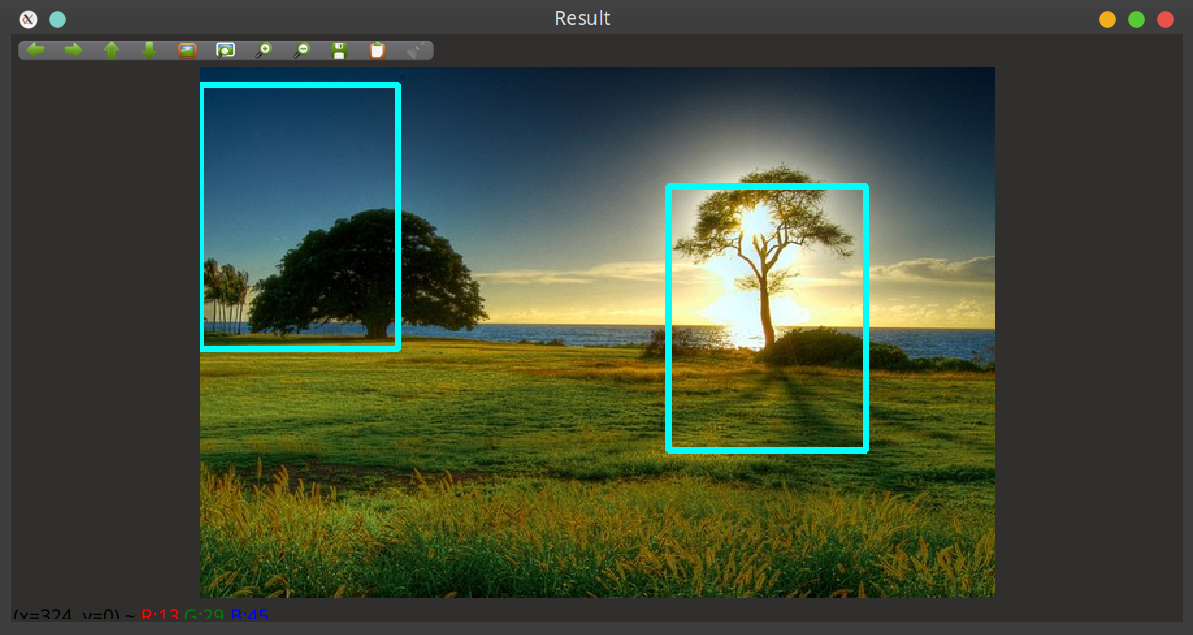
\includegraphics[width=6cm, height=4cm]{before/no_prep_0_48_0}
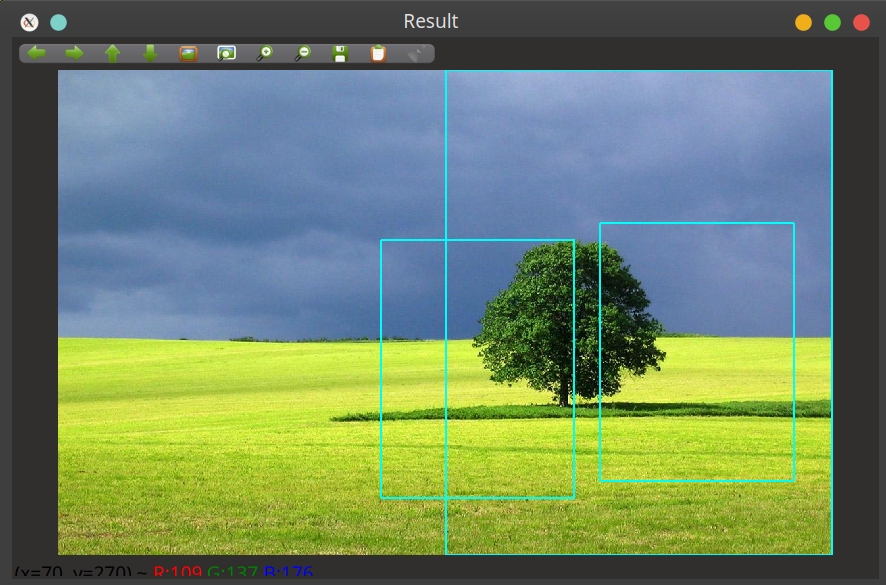
\includegraphics[width=6cm,height=4cm]{img/before/no_prep_0_48_1}
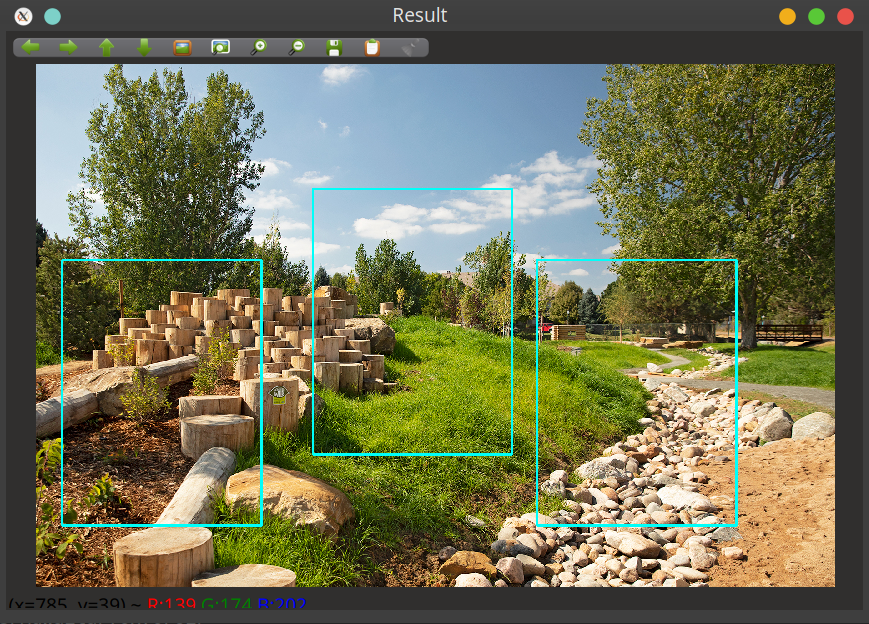
\includegraphics[width=6cm,height=4cm]{img/before/no_prep_0_48_2}
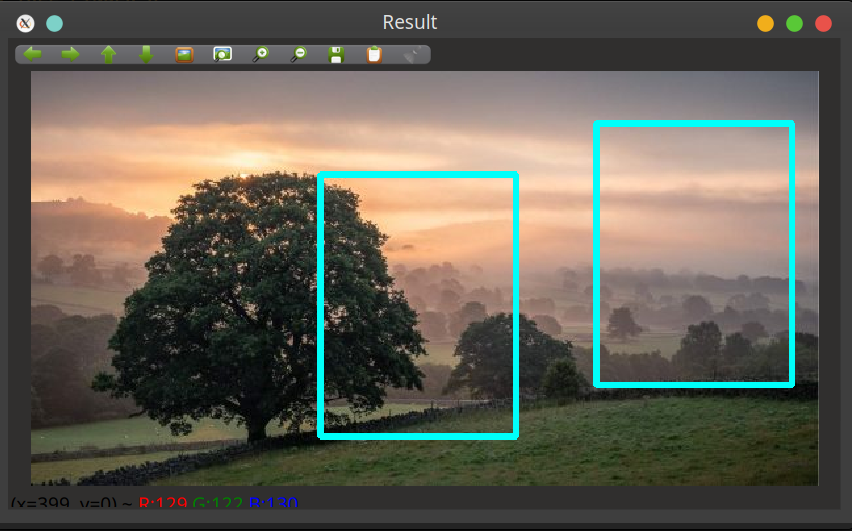
\includegraphics[width=6cm,height=4cm]{img/before/no_prep_0_48_5}
\end{center}

\vspace{0.5cm}

A parameter that greatly affected the quality of the results is the number of code-words computed from the set of features extracted from the training data-set. \\
The optimization of this parameter was made difficult by the time required for the training and the evaluation, that has to be done by a human: I didn't had a metric to automatically measure how far a detection was from the actual position of the tree.

On the other side, the confidence with a detection (i.e. the normalized distance from the margin) could be easily optimized as it can be changed without re-training the model.

\section{Reasoning about performance}
In many cases, like the top-right and bottom-right pictures of the previous section, trees were \textit{half}-located. 
\\
It seems that the windows containing trees gets discarded because there are too many \textit{green features} inside them, but when a few \textit{sky features} join the window then the position is accepted.

I tried to increase the number of code-words extracted to check if BoVW was able to better differentiate the features (e.g.  \textit{leaves features} from \textit{grass features}), but with poor results (obviously a larger dictionary requires a wider data-set).

After increasing the training data-set size up to 300 samples and testing many different configurations, I was demoralized by seeing that I couldn't get decent results.

How could I improve the localization? Is loosing relative features position ruining the detection?

I started thinking that BoVW is not suitable for this task.

\section{Issues investigation}
Rather than discarding the whole work and starting again from scratch, I decide to try having a deeper understanding of the key localization steps.

The training and test images have many different resolutions, ranging from 4000x1000 to 800x400. How does the behavior BoWV change, given two images of different resolution?

Checking the number of key-points inside a window wrapping a tree, I found that the undetected trees had a huge number of features compared to the correctly detected trees.
\\
For instance, comparing the following two testing images, I found that the tree in the left image (that is correctly detected) contains only 183/800 features, while the right image where the tree is not detected contains 5551/20 000 features! (see \textit{First implementation} section to check how these trees were localized).
\\
\begin{center}
	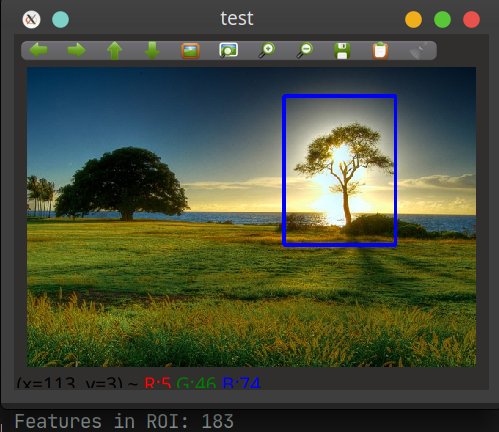
\includegraphics[width=6cm,height=4cm]{img/before/no_prep_0_48_nfeat}
	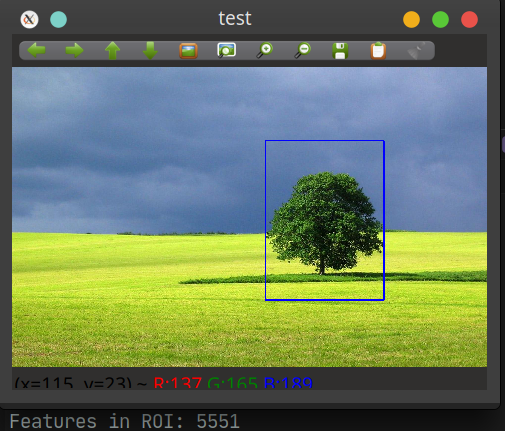
\includegraphics[width=6cm,height=4cm]{img/before/no_prep_0_48_1_n_feature}
\end{center}

The same observation applies to other miss-classified and correctly classified trees.

Is it possible that this huge number of features is \textit{fouling} the histogram vector that is input to the SVM (even if it is normalized)?
\\
With this idea in mind, I decide to try reducing the model complexity to see how its behavior changes.

\section{Second approach - complexity reduction}
The complexity reduction was achieved by reducing the input resolution:
\\
the model was trained using images rescaled to 400x300 and the sliding window approach was changed such that, for each window position:

\begin{enumerate}
	\item The window content is rescaled to 400x300 using bilinear interpolation
	\item A fresh set of features is extracted from the rescaled window
	\item The detection process is applied to the extracted features
\end{enumerate}

Finally, the number of dictionary code-words was reduced to 50.
The number of key-points found in each window position didn't exceed 300 features.

As expected the evaluation time of this new approach increased while the training time dropped from 20 minutes to less than 2 minutes, allowing a much faster testing. Thanks to the reduced training time I was able to quickly test different configurations, but unfortunately none of them was effective:

\vspace{0.5cm}

\begin{center}
	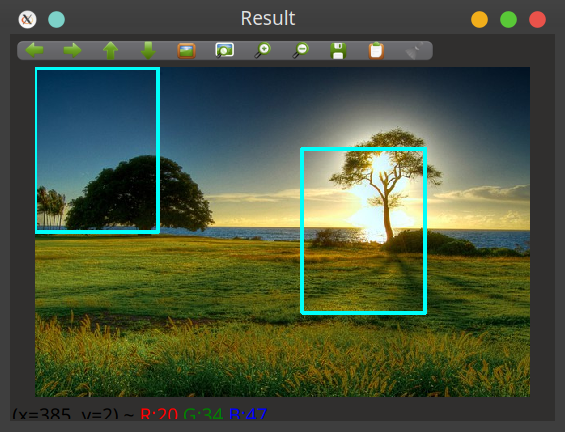
\includegraphics[width=6cm,height=4cm]{img/resized_window/Screenshot_20200707_191259}
	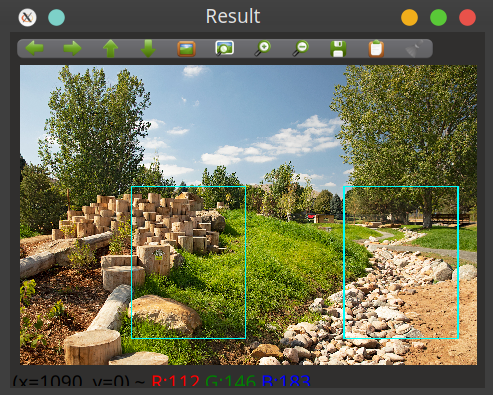
\includegraphics[width=6cm,height=4cm]{img/resized_window/Screenshot_20200707_191430}
	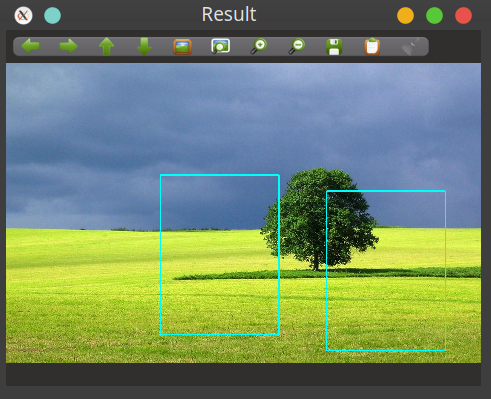
\includegraphics[width=6cm,height=4cm]{img/resized_window/Screenshot_20200707_191506}
	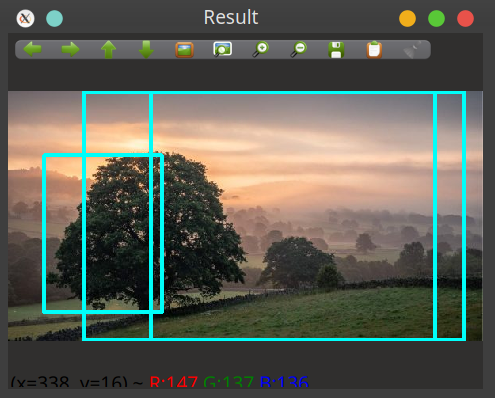
\includegraphics[width=6cm,height=4cm]{img/resized_window/Screenshot_20200707_191538}
	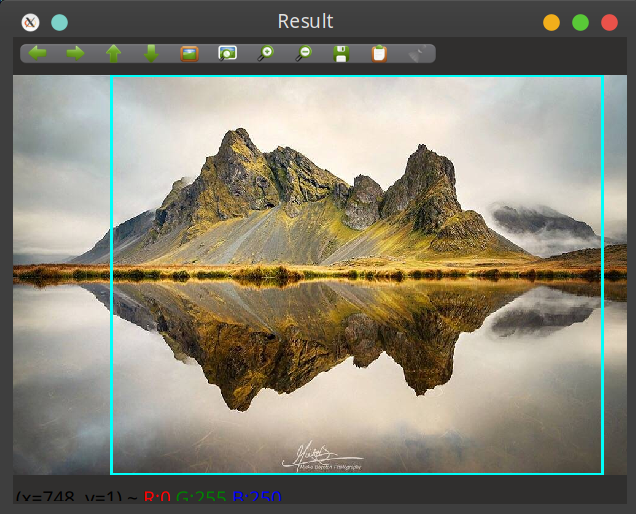
\includegraphics[width=6cm,height=4cm]{img/resized_window/Screenshot_20200707_191628}
\end{center}

\vspace{0.5cm}

Except for the top-left image, which is the one with the smallest resolution, there were many miss-classifications.

\section{Third approach - less drastic complexity reduction}
I decided to do one last try by mixing the first two approaches.

I'm still convinced that the variability of the input (resolution, different cameras...) affects the training, making the output model less stable.

Therefore I decided to follow this new approach: each training image, before being used, was resized to 1920x960. The initial localization process, where key-points are extracted once and then filtered by position, was restored.

Using a BoVW dictionary of 200 code-words the final result was sometimes decent but still far from accurate, as shown in the next section:\\
some locations contain trees, but are a bit shifted from the perfect locations. We can spot a few false positives and a very bad localization on the mid-right test image.

\section{Final results}

\vspace{0.5cm}
\begin{center}
	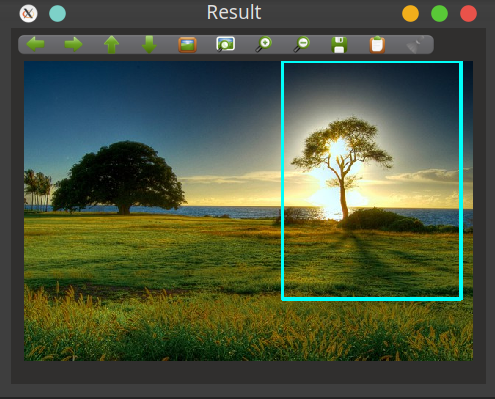
\includegraphics[width=10cm,height=6cm]{img/final/0}
\end{center}
\vspace{0.5cm}

The left tree is not recognized.

\vspace{0.5cm}
\begin{center}
	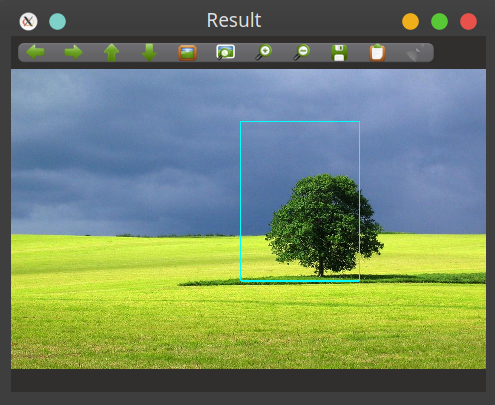
\includegraphics[width=10cm,height=6cm]{img/final/1}
\end{center}
\vspace{0.5cm}

The rectangle around the tree is a bit shifted from the best position: this is a consequence of Non Maxima Suppression and the score assigned to that window position (which is higher).

\vspace{0.5cm}
\begin{center}
	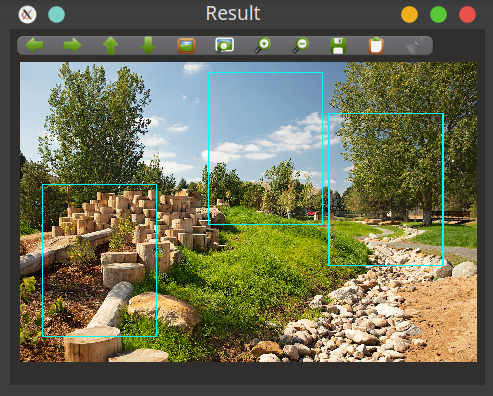
\includegraphics[width=10cm,height=6cm]{img/final/2}
\end{center}
\vspace{0.5cm}

Here we can spot one obvious false negative on the left. The rectangle on the right is not in the best position again due to a score difference.

\vspace{0.5cm}
\begin{center}
	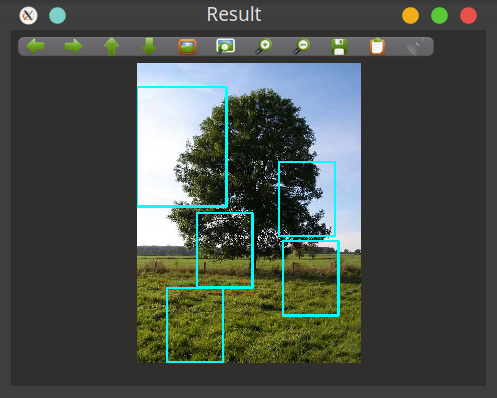
\includegraphics[width=10cm,height=6cm]{img/final/3}
\end{center}
\vspace{0.5cm}

This image has caused problems with many different configurations of parameters, highlighting that probably the training data-set can be improved a lot.

\vspace{0.5cm}
\begin{center}
	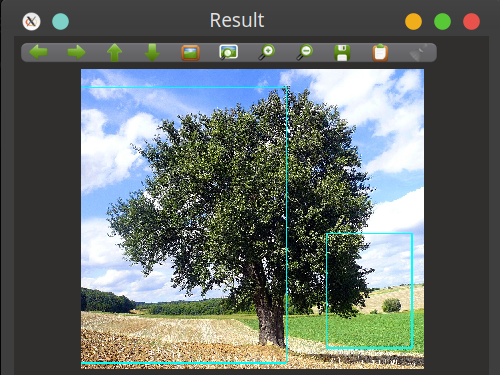
\includegraphics[width=10cm,height=6cm]{img/final/4}
\end{center}
\vspace{0.5cm}

While the left rectangle is shifted for the same reasons highlighted before, the right rectangle is a good example of why BoVW might not be sufficiently suitable for this task: by loosing relative feature position, a good amount of \textit{leaves features,} \textit{grass features} and \textit{sky features} are accepted.

\vspace{0.5cm}
\begin{center}
	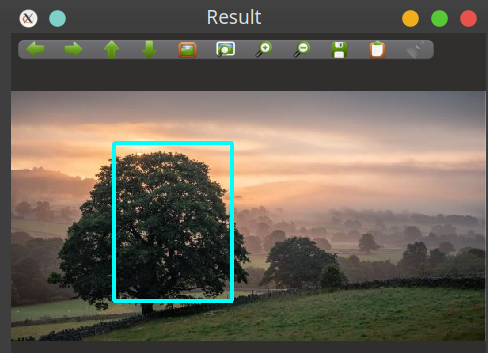
\includegraphics[width=10cm,height=6cm]{img/final/5}
\end{center}
\vspace{0.5cm}

Again, due to an higher score, the window not containing the whole tree is selected.

\vspace{0.5cm}
\begin{center}
	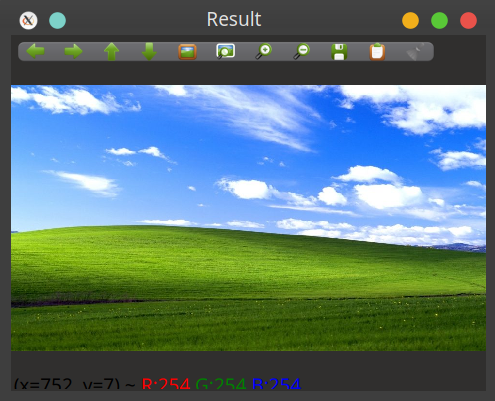
\includegraphics[width=10cm,height=6cm]{img/final/6}
\end{center}
\vspace{0.5cm}

This image initially contained false positives, but after adding \textit{grassland} images the problem no longer persisted.

\vspace{0.5cm}
\begin{center}
	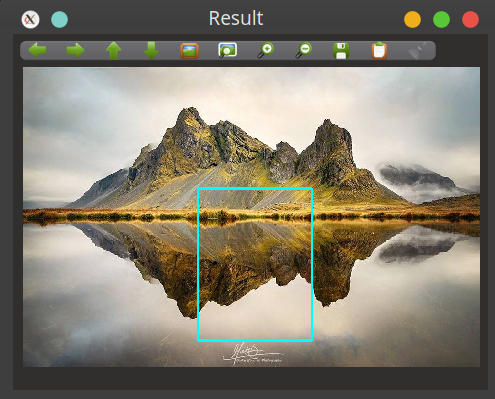
\includegraphics[width=10cm,height=6cm]{img/final/7}
\end{center}
\vspace{0.5cm}

Even by adding a few mountain images this picture is still miss-classified.

\vspace{0.5cm}
\begin{center}
	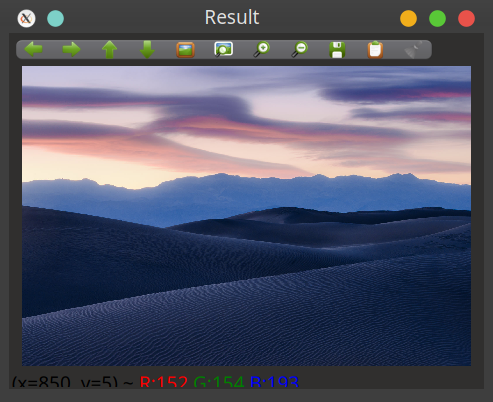
\includegraphics[width=10cm,height=6cm]{img/final/8}
\end{center}
\vspace{0.5cm}

This image didn't cause any problem from the beginning.

\vspace{0.5cm}
\begin{center}
	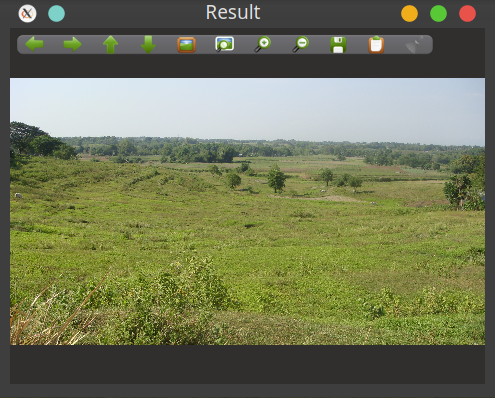
\includegraphics[width=10cm,height=6cm]{img/final/9}
\end{center}
\vspace{0.5cm}

Here the behavior is ideal: the small trees on the background are not detected.

\vspace{0.5cm}
\begin{center}
	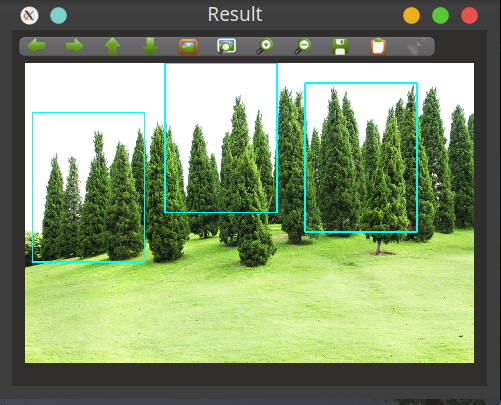
\includegraphics[width=10cm,height=6cm]{img/final/10}
\end{center}
\vspace{0.5cm}

The training data-set contains a few pine trees, in fact these trees are easily detected. However, the expected behavior would draw a rectangle around each of them, but this result is hard to achieve.

\vspace{0.5cm}
\begin{center}
	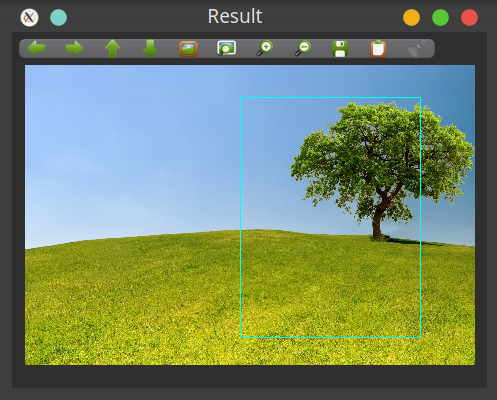
\includegraphics[width=10cm,height=6cm]{img/final/11}
\end{center}
\vspace{0.5cm}

The tree is almost perfectly detected, but the rectangle is a bit shifted from the best position for the same reasons explained before.

\vspace{0.5cm}
\begin{center}
	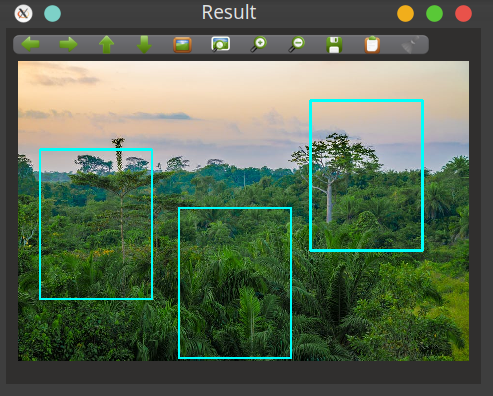
\includegraphics[width=10cm,height=6cm]{img/final/12}
\end{center}
\vspace{0.5cm}

This image is clearly hard, nevertheless it contains just one false positive.

\section{Conclusions}
The training data-set has shown to greatly influence the final model performance. Probably, the localization could be improved by refining that data-set and maybe adding some samples. Nevertheless, using the same camera hardware for capturing the training images and run the model would probably make it more stable and easier to control.

As it is implemented now, the localization process couldn't be used in real time applications. However the time required to evaluate an image could be greatly reduced by exploiting multi-threading, as different windows can be analyzed in parallel.

With these results, it seems that Bag of Visual Words is not the best suitable model to solve the task of detecting trees. The biggest issue with this method is the loss of relative position between features.\\
If I had to start from scratch, without using deep-learning, I would definitively try a cascade classifiers approach. \\
Anyway, besides the poor localization, during the development of the project I have faced a variety of issues from which I learned a lot.

\end{document}          
